%!TEX root = ../../dissertation.tex

\section{Motivation} % (fold)
\label{sec:motivation}

As technology evolves people have more powerful devices and they want to take advantage of that. They want to have more realistic experiences with larger, more detailed and complex contents.
This is observable in the graphic contents. With the recent extra high definition on screens and the computational power of the machines beating records, the graphic content has to follow up that characteristics in quantity as well as in quality. The issue is that the manual content generation takes a long work time from artists to achieve this quality, which implies high costs.

Graphic contents are mainly used for entertainment, both in the gaming and movie industries, but they are also used in many other different areas. The fields of architecture and design, for instance, use this technology to experiment and model new designs, from small objects like a plate, to buildings or even entire cities. Unfortunately, manual modeling of large sets of potentially complex shapes is tiresome and very costly. 

Figure~\ref{fig:brickwall} is a wall that has a relatively large amount of objects (bricks). Here each brick has to be modeled one by one and positioned in its place. Which is a rather complex work because each brick has different positions and rotations. This example shows that from a set of simple objects, such as the ones that compose this model, a complex model can be produced, and the manual modeling of this type of models is a complex, error prone, and time consuming process.

\begin{figure}[htbp]
	\centering
	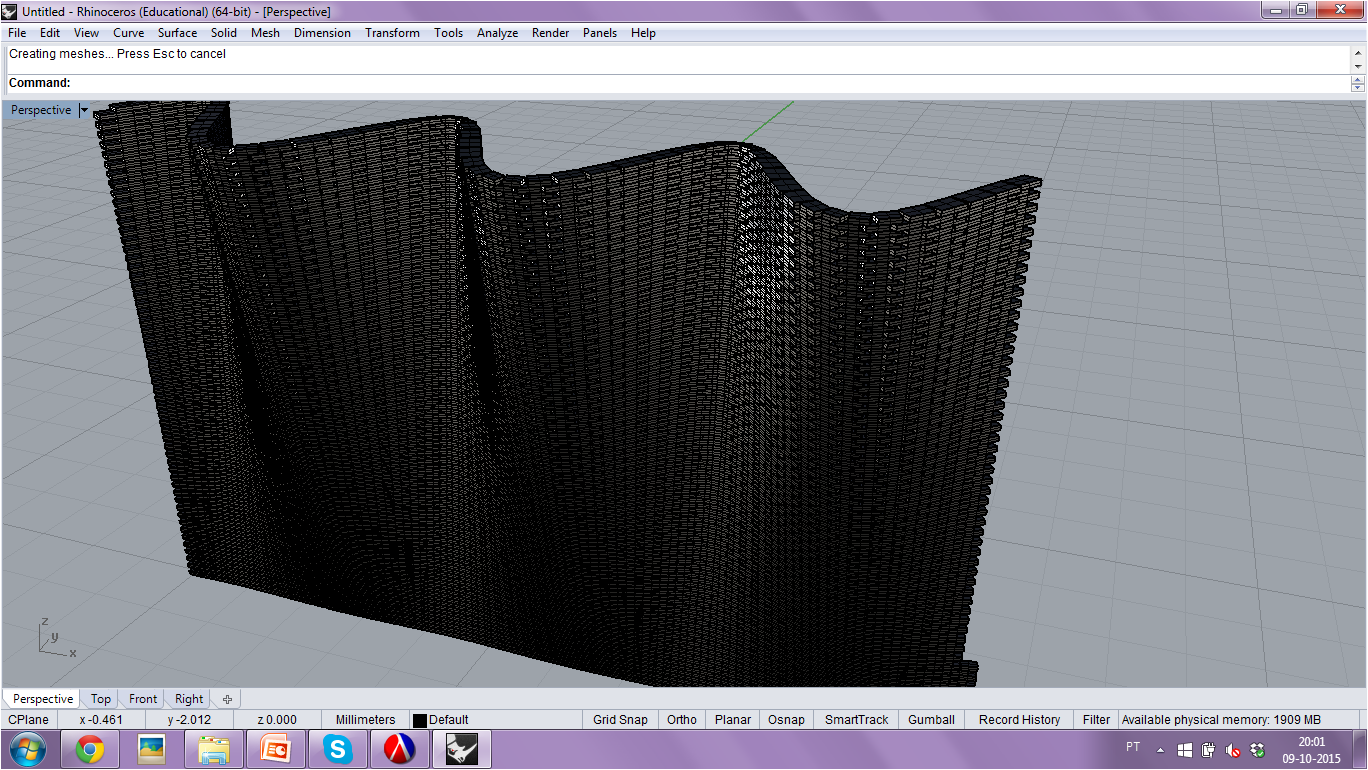
\includegraphics[width=0.7\textwidth, trim = 20mm 25mm 80mm 28mm, clip]{images/parede-sin.png}
	\caption{Wall of bricks}
	\label{fig:brickwall}
\end{figure}


%In this field they also face the problems that raises from the modeling of really big sets of objects and forms manually, which is slow and error prone. 
%\emph{This work addresses the problem of large content creation and will focus on the fields of architecture and design.}

The obvious solution to this problem is to hire more architects or designers in order to increase productivity and reduce the time needed. However, experience has shown that this solution is not scalable, i.e. doubling the number of architects or designers working in a project will not double their overall productivity. Also, this solution has a big impact on financial costs, that would take immediately out of the market producers with fewer resources.

A solution for this problem is the use of \gls{GD}. It is a design method that is based on a programming approach which allows architects and designers to model large volumes of complex shapes with significantly less effort. They can model cities, buildings, trees, and many other objects that are, usually, too big or complex for a manual approach. Since the models are represented by a computer program, large volumes of geometry can be generated within short periods of time. This is positive to the users because it is more efficient than the manual approach, but, in the other hand, it imposes the use of machines with performance that can handle large amounts of geometry fast. The brick wall model (Figure~\ref{fig:brickwall}) can be easily modeled, with a \gls{GD} approach by using a sinusoidal function for the positioning of the bricks. 

Although most \gls{CAD} applications provide programming languages for generative design, programs written in these languages have very limited portability. Additionally, the provided languages, such as AutoLisp, C++ or Visual Basic, are not pedagogical and are difficult to use even to experienced programmers. All this problems create barriers to the adherence to this approach by all users, specially those that are not used to code.\cite{ramos_et_al:OASIcs:2014:4565}

There are several generative design (GD) tools such as Grasshopper\footnote{\url{http://www.grasshopper3d.com/}} and Rosetta\cite{Leit2012}, that aim to break down some of this barriers, and facilitate the approximation of these individuals to programming. With this tools the users can create their models using pedagogical and easy to use languages. This systems implement a straightforward pipeline presented in Figure~\ref{fig:GD_Pipeline}.


%\begin{figure}[htbp]
%	\centering
%	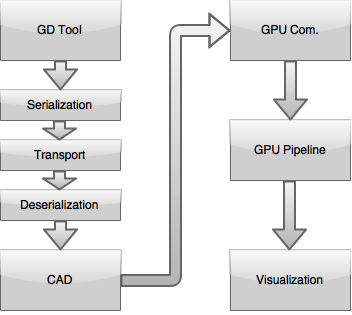
\includegraphics[width=0.45\textwidth]{images/Architecture/GD-Common-Pipeline.png}
%	\caption{Common Generative Design Pipeline}
%	\label{fig:GD_Pipeline}
%\end{figure}

However, there is a problem: CAD applications are built for manual modeling mainly, and are not prepared to quickly handle large amounts of geometry.
Users implement their models through the GD tool interface. Then all the geometry data is serialized and the data is transfered through some transport mechanism. This data has to be deserialized on the other side within the CAD application. The CAD application takes the deserializes data and processes it producing geometry. Finally, the geometry is moved to the GPU that renders it. All these steps are time-consuming, due to the large amount of data that needs to be transfered and processed within each step. With this rises a performance problem.

One big difference between GD and traditional approaches is that users do not see the result of their program while they code. They follow a code-execute-visualize loop where they make changes in the code, execute the code and visualize the resulting model. This makes it difficult for them to understand the impact of changes in their programs, which is worst if they have to wait much time to visualize it. It would be much more productive if they could easily understand the correlation between their program and the resulting model and to be able to experiment values on their program and see the effects they have on the model. To help them with this, there is the concept of \emph{immediate feedback}. Immediate feedback is a mechanism that allows the users to quickly see the results of the changes they make. This can be implemented, for instance, through the use of sliders that can be associated with values on the program, and when one slider is moved the effects of that change should be visualized immediately. 

Running the code produces much more geometry and much faster than manual modeling, so the user is able to create massive amounts of geometry, which is fed to the CAD that gets overloaded. With this issues, it is hard to get good performance, specially with large models, that makes impossible to have true immediate feedback. There are a lot of techniques that architects and designers may want to use, such as Fractals(Section~\ref{ssub:fractals}), Cellular Automata (Section~\ref{sub:cellular_automaton}), and L-Systems (Section~\ref{ssub:l_systems}), that can generate large amounts of geometry from simple sets of instructions. The use of this techniques are not possible with manual use, due to the large amount of geometry, and is also not possible with the normal pipeline because its performance can not handle the massive amount of geometry that is generated.


This work proposes a solution to this problem and aim to generate large volumes of geometry that is as close as possible to real-time. It does so by jumping over some steps while drastically decreasing the amount of data that is transfered between steps. First we aim to get the geometry as fast as possible to the GPU, so since our goal is just visualization, we jump the CAD layer, eliminating the first communication steps. Another action is to reduce the amount of data that is transferred, by transferring only a very concise description of the geometry, generating the actual geometry on the GPU.
To improve visualization performance, techniques such as Level Of Detail (Section~\ref{sub:level_of_detail}) and Occlusion Culling (Section~\ref{sub:occlusion_culling}) are explored.

The processing work for the generation and visualization of the geometry is shared between the \gls{CPU} and the \gls{GPU}. Happens that the work load can be splitted between this two elements in various different ways. And we explore some different ways to aim to have the best performance possible.
The most common solutions assign the large part of the load to the \gls{CPU}, that is responsible for fully generate the geometry which is then sent to the \gls{GPU} that just does pay off.

The simplest and most used load distribution is to assign a large part of it to the \gls{CPU}, where all the geometry is generated which results in a polygon mesh that is fed to the \gls{GPU}. The \gls{GPU} just renders the final result without any processing of the geometry.

It is also possible to give some of the work to the \gls{GPU}. This is done taking advantage of the programmable \gls{GPU}s, where we can use their processing power to manipulate or generate geometry. The \gls{GPU} is able to execute programs, called shaders, that are able to manipulate the geometry that is generated by the \gls{CPU}. With this method, the geometry is generated by the \gls{CPU} but it is changed by the \gls{GPU}. The \gls{GPU} is able to improve detail of the meshes or implement light effects, among other things.

One alternative to the last distribution is to assign a larger part of the processing work to \gls{GPU}. With this distribution the \gls{CPU} creates concise descriptions of the geometry, which is lighter work load, and the \gls{GPU} is responsible for the amplification of the geometry from the descriptions.

The last alternative is to assign most of the work to the \gls{GPU}. With this method, the program that generates the geometry is fully executed by the \gls{GPU}. It is the option that is more complex since all the code have to be written or translated to shader code. Because it runs only on the \gls{GPU}, we can take advantage of the large number of processors that the \gls{GPU}s currently have, and with that get performance improvements.


% section motivation (end)

